%% results_05a_rq1.tex
%% User Story 1: Dimensionality Scaling
%% All numbers come from results_converters/rq1_results_converter.py run on
%% RQ1+RQ2/results_config-dimensionality.csv (6,720 rows) and
%% results_config-dimensionality-extreme.csv (28 rows).
%% Figures: latex/figures/rq1_f*.pdf
%% ============================================================

\subsection{User Story 1: Dimensionality Scaling}
\label{sec:us1}

\paragraph{Research question.}
\emph{``As a user with a dataset that has many features, I want to find the
fastest model-agnostic library for high-dimensional datasets.''}

\paragraph{Experimental design.}
We evaluated seven method configurations---SHAP kernel and permutation,
\shapiq\ kernel and permutation, LightSHAP kernel and permutation, and
DALEX permutation---across four datasets at three feature counts each
(ames\_housing: 14/32/79; covertype: 14/28/54; diabetes\_130: 14/24/47;
gisette: 14/64/256), four model types, two budget levels (512 and 1\,024
coalition evaluations), and ten random seeds, yielding 6\,720 benchmark
runs in total.
All methods are approximate: this experiment contains no exact Shapley
reference, so quality metrics reflect \emph{cross-method agreement}, not
accuracy against a ground truth.
A hard 10-minute execution cap was applied per run.

% ── Runtime scaling ────────────────────────────────────────────────────────────
\subsubsection{Runtime Scaling by Feature Count}

\begin{figure}[ht]
  \centering
  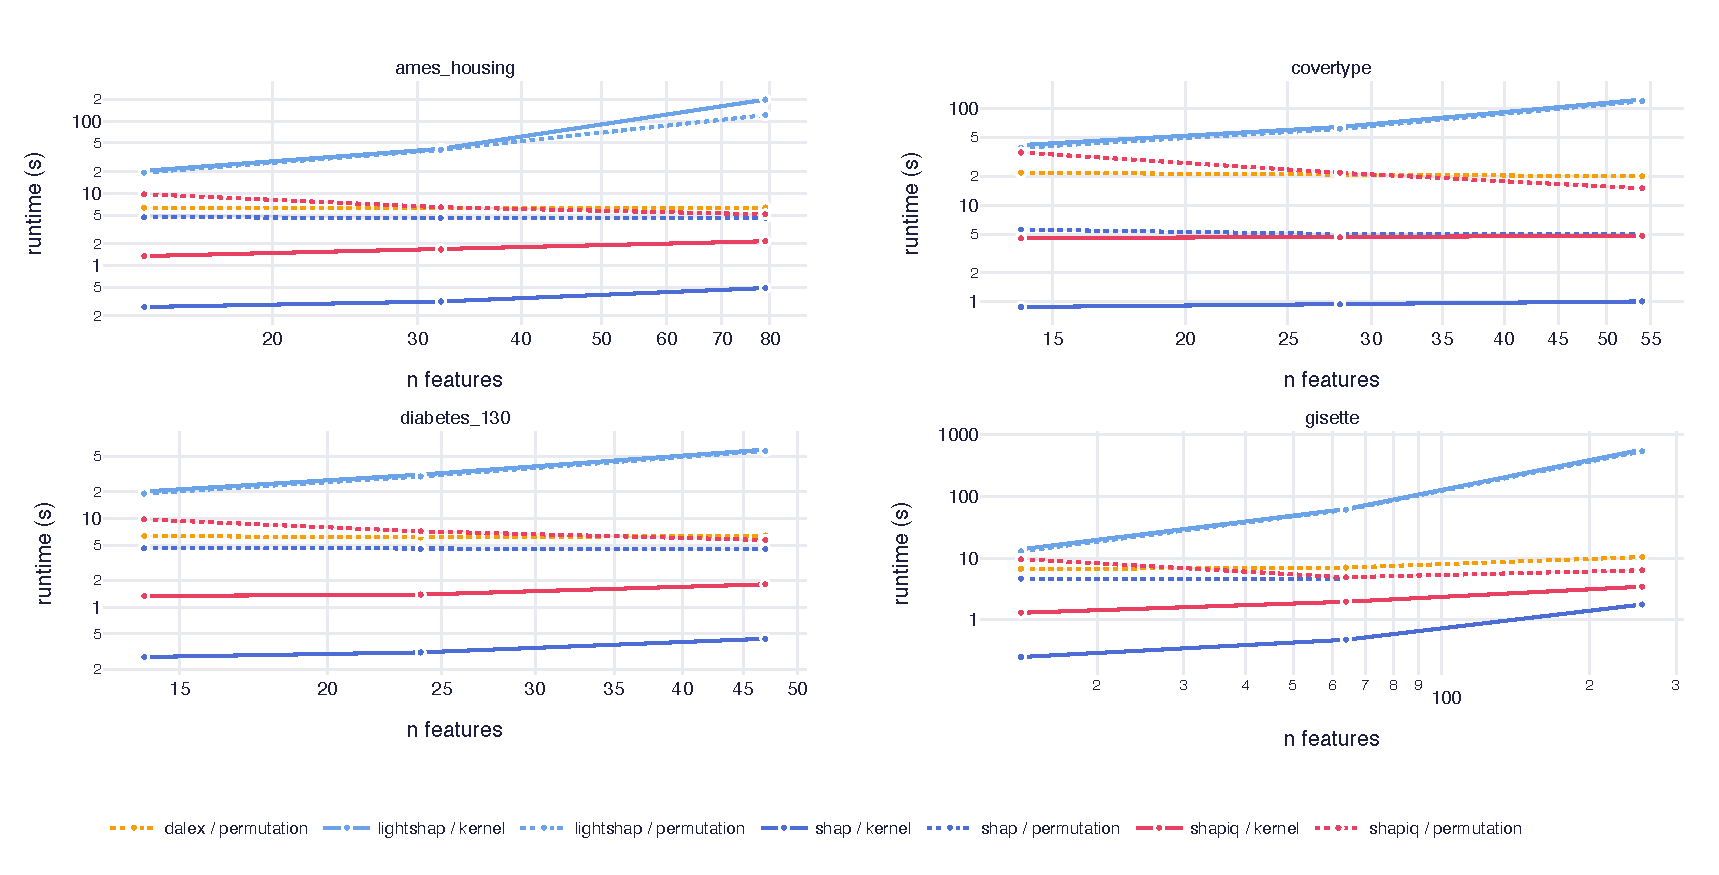
\includegraphics[width=\linewidth]{figures/rq1_f1_runtime_scaling}
  \caption{%
    Median runtime (seconds, log--log scale) vs.\ number of features for all
    seven method configurations at budget~512, split by dataset
    (each dataset uses its own feature grid).
    Lines are medians over four models and ten seeds; shaded bands show the
    interquartile range across seeds.
    Time-capped runs ($\geq$595\,s) are excluded from medians;
    they appear in Figure~\ref{fig:rq1-infeasibility}.
  }
  \label{fig:rq1-scaling}
\end{figure}

Figure~\ref{fig:rq1-scaling} shows the scaling trajectories across all four
datasets.
At 14 features, SHAP kernel is the fastest method with a median runtime of
0.26\,s; LightSHAP variants are the slowest at 16--17\,s.
The relative order shifts substantially with dimensionality: at 256 features
(gisette, budget 1\,024, time-capped runs excluded), SHAP kernel (3.6\,s)
and \shapiq\ kernel (5.2\,s) remain the most efficient, while DALEX
permutation reaches 20.6\,s.

Across all four datasets, SHAP kernel and \shapiq\ kernel exhibit the flattest
scaling slopes in log--log space, indicating near-linear growth in the number
of evaluated coalitions.
DALEX permutation and both LightSHAP variants show steeper growth, with
LightSHAP becoming infeasible at high feature counts (see
Section~\ref{sec:rq1-feasibility}).

% ── Budget effect ─────────────────────────────────────────────────────────────
\subsubsection{Budget Effect on Runtime}

\begin{figure}[ht]
  \centering
  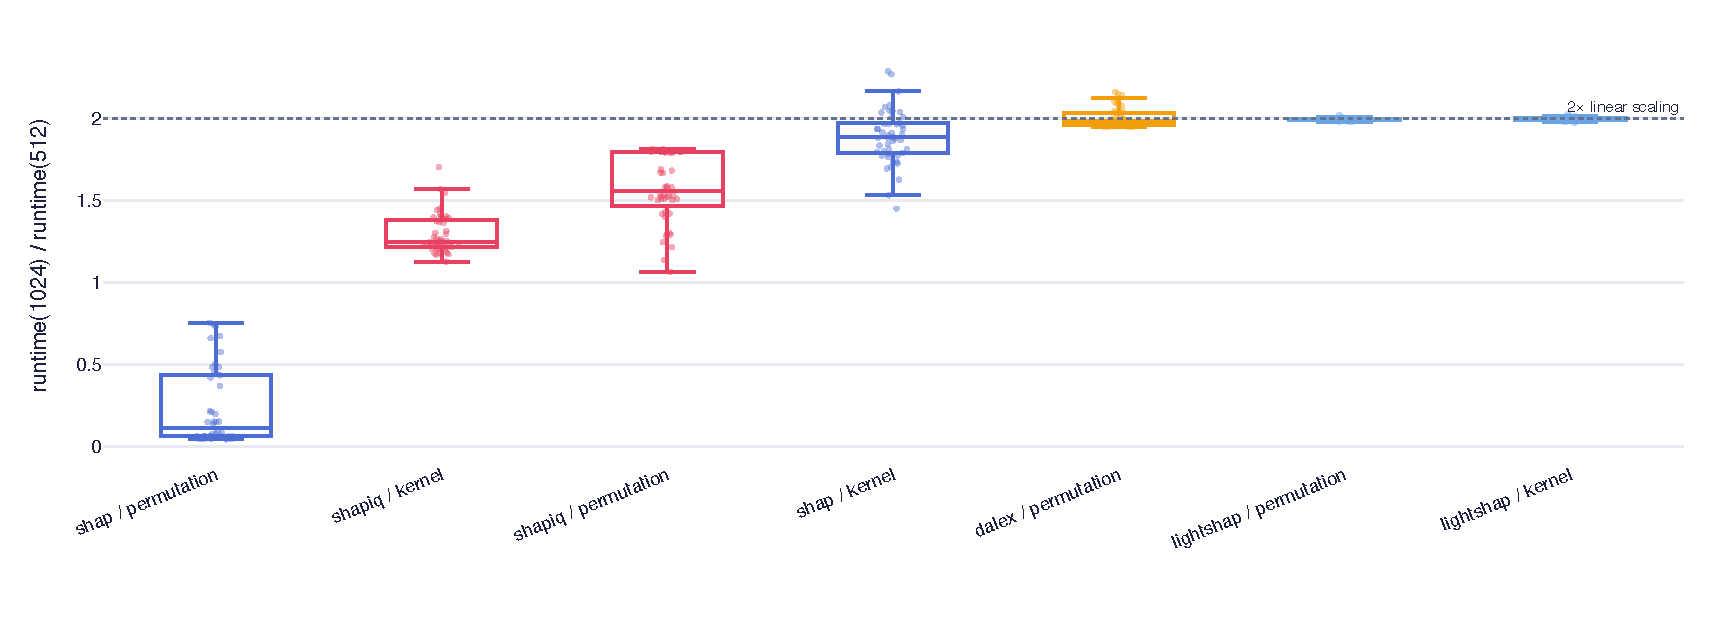
\includegraphics[width=\linewidth]{figures/rq1_f2_budget_ratio}
  \caption{%
    Distribution of the runtime ratio $t_{1024}/t_{512}$ per method, computed
    per dataset~$\times$~model~$\times$~feature-count cell.
    Each point is one experiment cell; the dotted line marks the
    2$\times$ ratio expected under purely linear budget scaling.
    Configurations where either budget's median runtime was unavailable
    (all runs capped or failed) are excluded.
  }
  \label{fig:rq1-budget}
\end{figure}

For a pure sampling method, doubling the budget should double the runtime
(ratio $\approx 2$).
Figure~\ref{fig:rq1-budget} shows that SHAP kernel, \shapiq\ kernel, and
DALEX permutation cluster closely around the 2$\times$ line, confirming
near-linear scaling in budget for these methods.
LightSHAP and the permutation variants of SHAP and \shapiq\ show wider
spread, with some cells below 2 (fixed overhead dominates) and others above
(superlinear growth at high feature counts).

% ── Feasibility ───────────────────────────────────────────────────────────────
\subsubsection{Execution-Cap Feasibility}
\label{sec:rq1-feasibility}

\begin{figure}[ht]
  \centering
  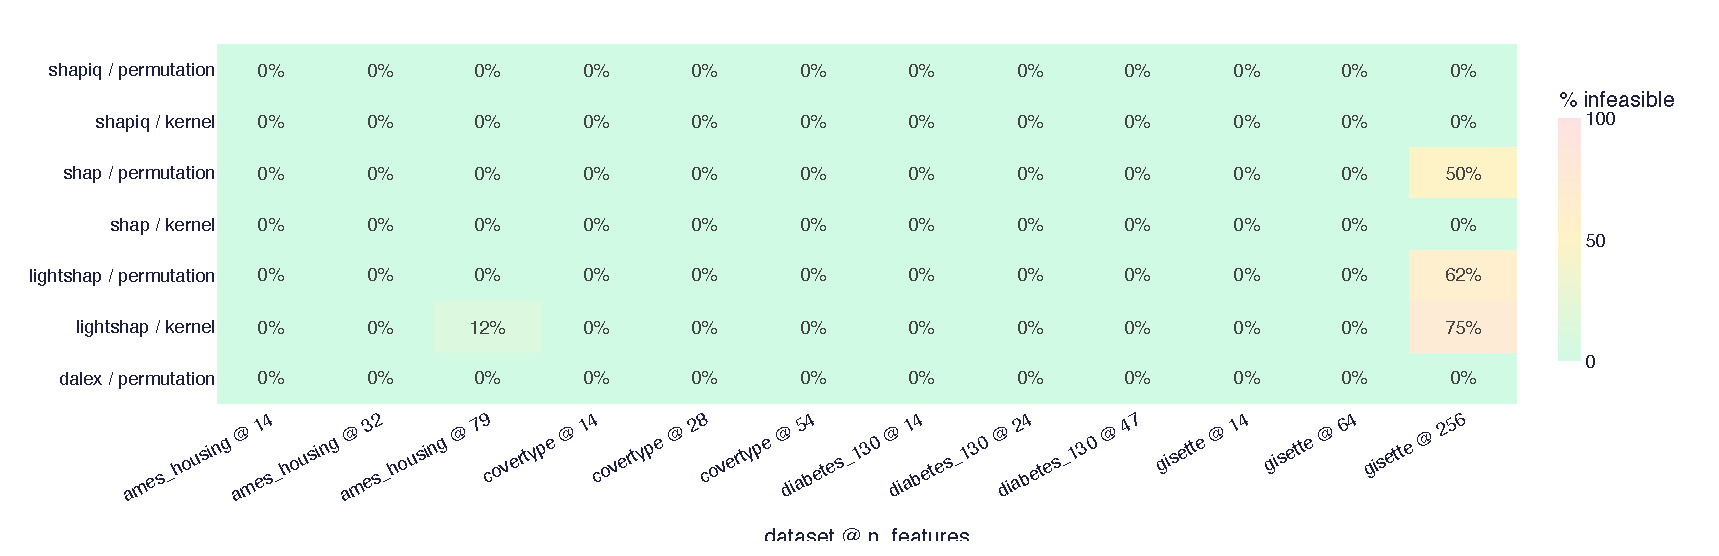
\includegraphics[width=\linewidth]{figures/rq1_f3_infeasibility}
  \caption{%
    Fraction of infeasible runs per method and dataset--feature-count cell.
    \emph{Infeasible} pools two distinct failure modes:
    (1)~\emph{time-capped} runs that hit the 10-minute wall-clock limit
    (all LightSHAP); and
    (2)~\emph{failed} runs that returned no output because the requested
    budget fell below the minimum required to complete one permutation pass
    ($2M+2 = 514$ evaluations at $M=256$ features, exceeded by budget~512;
    affects SHAP permutation only).
    The denominator per cell is 80 runs
    (4 models~$\times$~2 budgets~$\times$~10 seeds).
  }
  \label{fig:rq1-infeasibility}
\end{figure}

Figure~\ref{fig:rq1-infeasibility} reveals two qualitatively different
failure modes.
\textbf{LightSHAP} is the only library affected by the time cap: at
256 features in the gisette dataset, 75\,\% of LightSHAP kernel runs and
62.5\,\% of LightSHAP permutation runs exceed the 10-minute limit; at
79 features (ames\_housing), 12.5\,\% of LightSHAP kernel runs are capped.
\textbf{SHAP permutation} at 256 features fails structurally at budget~512:
one permutation pass requires $2M+2 = 514$ model evaluations, which exceeds
the 512-evaluation budget, so the explainer returns immediately with no
output (50\,\% of cells, since budget 1\,024 succeeds).
All other library--feature-count combinations complete successfully within
the 10-minute window.

\finding{%
  LightSHAP is the only library with a time-feasibility problem in the
  standard benchmark; it fails to finish in 10\,min for 62--75\,\% of
  runs at 256 features.
  SHAP permutation has a structural budget constraint: budget~512 is
  insufficient at $M \geq 257$ features.
  All remaining configurations (SHAP kernel, \shapiq, DALEX) complete
  reliably across the tested range.%
}

% ── 1,000-feature stress test ─────────────────────────────────────────────────
\subsubsection{Extreme Dimensionality: 1,000-Feature Stress Test}
\label{sec:rq1-stress}

\begin{figure}[ht]
  \centering
  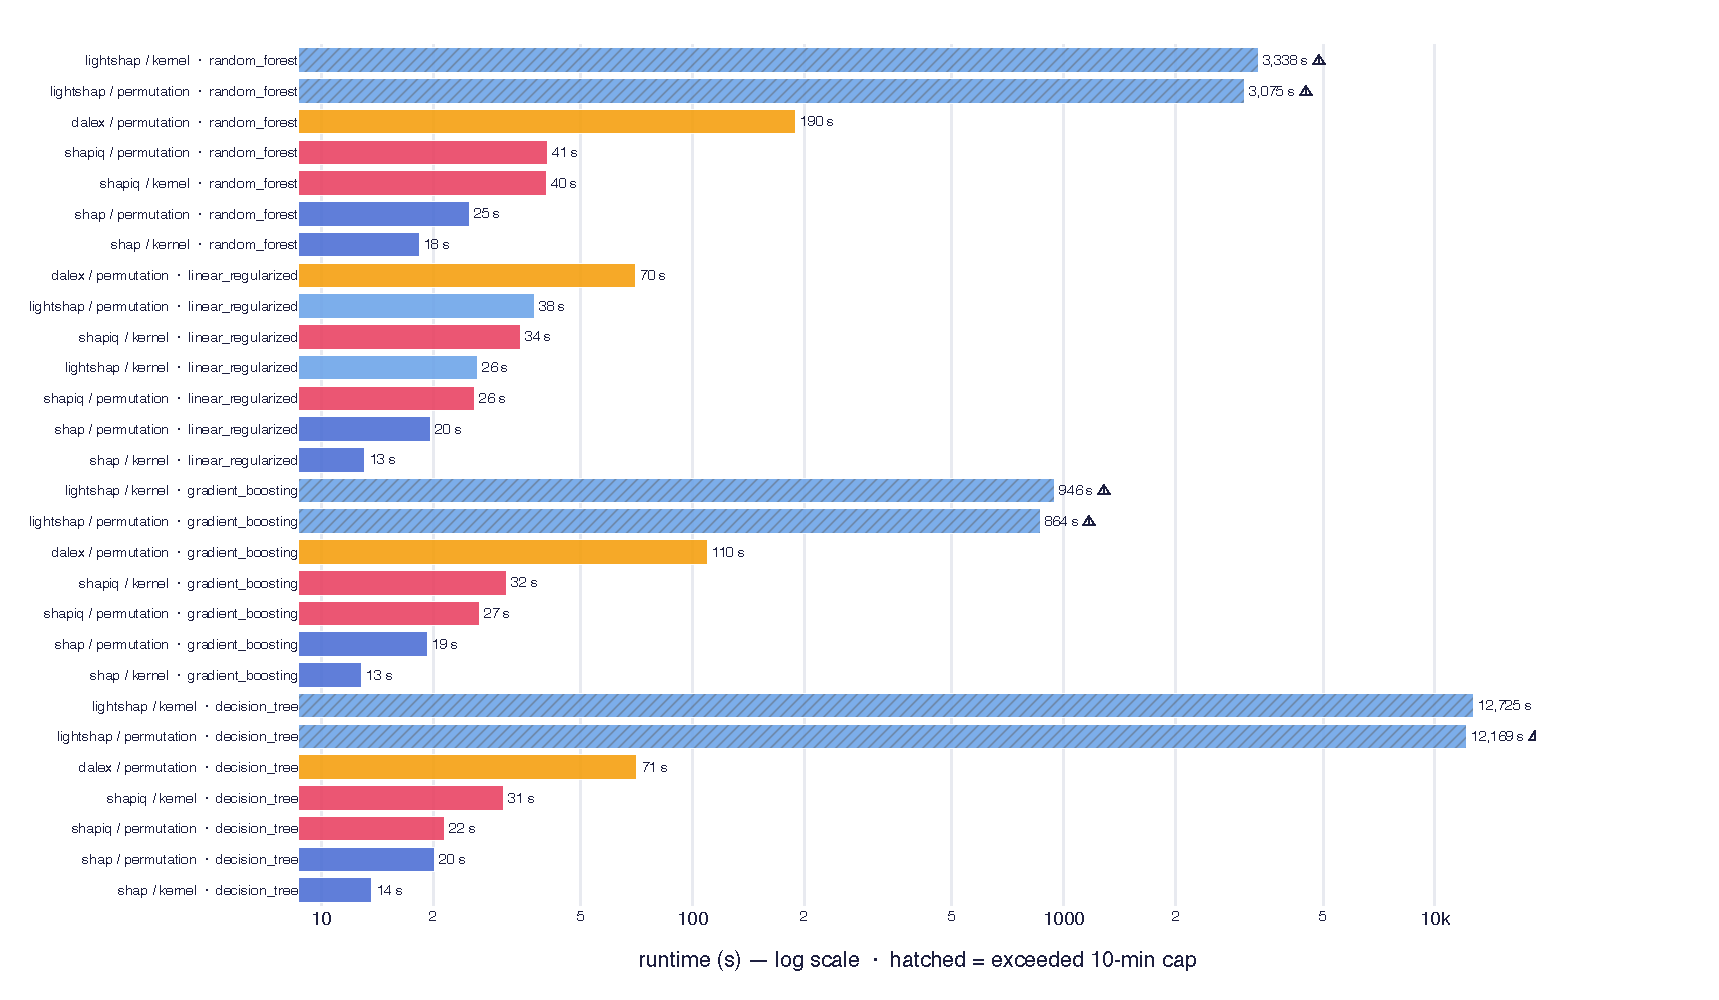
\includegraphics[width=\linewidth]{figures/rq1_f5_stress_test}
  \caption{%
    Wall-clock runtime for all seven methods across four models on the
    gisette dataset at 1\,000 features (budget~2\,048, seed~0 only).
    Hatched bars indicate runs that exceeded the 10-minute execution cap
    (actual wall-clock time recorded up to $\approx$3.5\,h).
    This is a \emph{one-shot feasibility stress test}; its results are not
    comparable with the standard scaling curves in
    Figure~\ref{fig:rq1-scaling} (different dataset scope, seed count,
    and budget).
  }
  \label{fig:rq1-stress}
\end{figure}

Table~\ref{tab:stress} summarises the extreme stress test.
SHAP kernel is the only method that remains computationally tractable across
all four model types at 1\,000 features, with runtimes between 12.9\,s
(gradient boosting) and 18.4\,s (random forest).
All LightSHAP runs exceed the 10-minute cap, reaching up to 3.5\,h for
decision tree models.
\shapiq\ and DALEX permutation require 20--71\,s and 32--71\,s respectively,
remaining practical for most models.

\begin{table}[ht]
  \centering
  \caption{%
    Runtimes at 1\,000 features (gisette, budget~2\,048, seed~0).
    $\dagger$ = exceeded 10-minute execution cap; value is actual wall-clock.
  }
  \label{tab:stress}
  \begin{tabular}{lrrrr}
    \toprule
    Method & \multicolumn{4}{c}{Runtime (s) by model} \\
    \cmidrule(lr){2-5}
           & Decision tree & Grad.\ boost. & Linear & Random forest \\
    \midrule
    SHAP kernel        & 13.7 & 12.9 & 13.1 & 18.4 \\
    SHAP permutation   & 21.9 & 19.4 & 14.8 & 22.0 \\
    \shapiq\ kernel    & 26.4 & 20.9 & 34.2 & 46.7 \\
    \shapiq\ permutation & 30.7 & 26.6 & 26.2 & 41.1 \\
    DALEX permutation  & 71.4 & 70.3 & 70.1 & 71.4 \\
    LightSHAP kernel   & \phantom{0}12{,}725$\dagger$ & \phantom{00}946$\dagger$ & \phantom{00}--- & \phantom{0}3{,}338$\dagger$ \\
    LightSHAP permutation & \phantom{0}12{,}169$\dagger$ & \phantom{00}864$\dagger$ & \phantom{00}--- & \phantom{0}3{,}075$\dagger$ \\
    \bottomrule
  \end{tabular}
\end{table}

\finding{%
  At 1\,000 features, SHAP kernel is the only method to complete within
  one minute across all model types.
  LightSHAP is infeasible at this dimensionality (all runs exceed 10\,min,
  up to 3.5\,h for tree models).
  \shapiq\ and DALEX permutation remain practical ($<$72\,s).%
}
